\documentclass[12pt, twoside]{article}
\usepackage[francais]{babel}
\usepackage[T1]{fontenc}
\usepackage[latin1]{inputenc}
\usepackage[left=7mm, right=7mm, top=7mm, bottom=7mm]{geometry}
\usepackage{float}
\usepackage{graphicx}
\usepackage{array}
\usepackage{multirow}
\usepackage{amsmath,amssymb,mathrsfs}
\usepackage{soul}
\usepackage{textcomp}
\usepackage{eurosym}
 \usepackage{variations}
\usepackage{tabvar}

\pagestyle{empty}

\begin{document}

\begin{flushleft}
NOM PRENOM: \ldots \ldots \ldots \ldots \ldots \ldots \ldots \ldots \ldots
 
\bigskip

\end{flushleft}

\begin{center}
{\fbox{$4^{e}4$ \qquad \qquad \textbf{\Large{Mini-test 2 (sujet 1)}}
\qquad \qquad \ldots/12/2014}}
\end{center}



\bigskip

\textit{Remarque: Tout le contr�le est � faire sur cette feuille. Laisser vos
traits de constructions. Codage et pr�cision sont pris en compte.}

\medskip

\begin{enumerate}
  
  \item Donner la d�finition de m�diane d'un triangle. (\textit{1,5 point})
  
  \rule{18cm}{0.5pt}
  

  \rule{18cm}{0.5pt}
   
   
   
   \rule{18cm}{0.5pt}
    
    
    \enskip
    
  \item 
  
  Construire la m�diatrice du segment [AB] en utilisant
  l'�querre. (\textit{1,5 point})
  
  \bigskip
  
  \begin{center}
  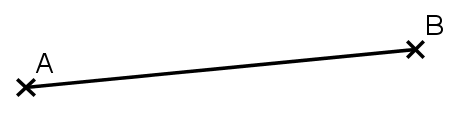
\includegraphics[width=6cm]{images/media1.png}
  \end{center}

\bigskip

  \item Construire la m�diatrice de [CD] en utilisant le compas (sans
  l'�querre). (\textit{1,5 point})
  
\bigskip

\bigskip
  
  \begin{center}
  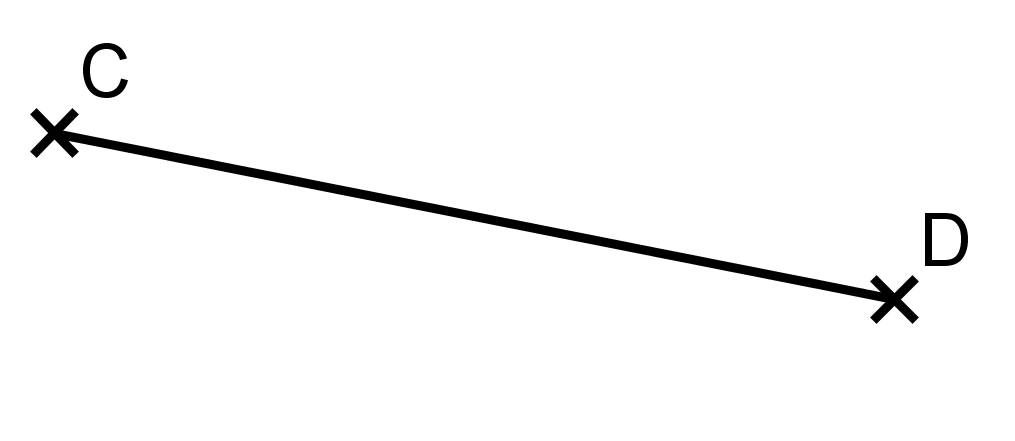
\includegraphics[width=4cm]{images/media2.png}
  \end{center}  

\bigskip
  
  \item 
  
 \begin{tabular}{cc}
 \begin{minipage}{12cm}
 ABC est un triangle rectangle en A. Tracer son cercle circonscrit (vous
  utiliserez la m�thode de votre choix). (\textit{2,5 points})

 \end{minipage}
&
 \begin{minipage}{6cm}
 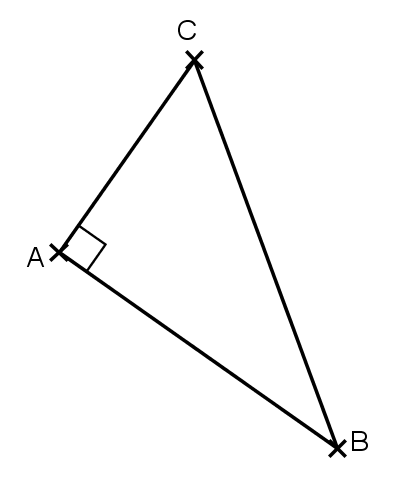
\includegraphics[width=5cm]{images/triangle.png} 
 \end{minipage}
 \end{tabular} 
 
  
  



  \item $\mathcal{C}$ est un cercle de diam�tre [UV] et W est un point du
  cercle.
  
   \begin{tabular}{cc}
 \begin{minipage}{12cm}
 \begin{enumerate}

    \item  Que peut-on dire du triangle UVW? (\textit{1 point})
    
    \rule{10cm}{0,5pt}
    
     \rule{10cm}{0,5pt}
    
    \item Citer la propri�t� du cours permettant de l'affirmer 
    
    (\textit{1,5
    point}):
    
    \rule{10cm}{0,5pt}
    
    \rule{10cm}{0,5pt}
    
    \rule{10cm}{0,5pt}
    
    \rule{10cm}{0,5pt}
    
     \rule{10cm}{0,5pt}
     
    
  \end{enumerate}
 \end{minipage} 
&
\begin{minipage}{6cm}
 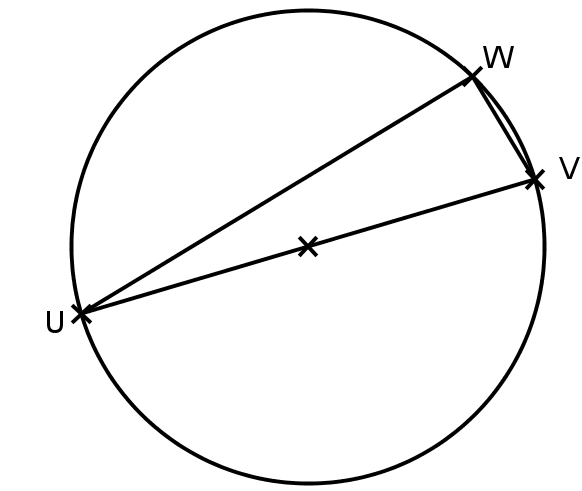
\includegraphics[width=6cm]{images/cercle.png} 
 \end{minipage} 
\end{tabular}

 \end{enumerate}

\pagebreak



\begin{flushleft}
NOM PRENOM: \ldots \ldots \ldots \ldots \ldots \ldots \ldots \ldots \ldots
 
\bigskip

\end{flushleft}

\begin{center}
{\fbox{$4^{e}4$ \qquad \qquad \textbf{\Large{Mini-test 2(sujet 2)}}
\qquad \qquad \ldots/12/2014}}
\end{center}



\bigskip

\textit{Remarque: Tout le contr�le est � faire sur cette feuille. Laisser vos
traits de constructions. Codage et pr�cision sont pris en compte.}

\medskip

\begin{enumerate}
  
  \item Donner la d�finition de m�diane d'un triangle. (\textit{1,5 point})
  
  \rule{18cm}{0.5pt}
  

  \rule{18cm}{0.5pt}
   
   
   
   \rule{18cm}{0.5pt}
    
    
    \enskip
    
    
    
  \item 
  
  Construire la m�diatrice du segment [AB] en utilisant le
  compas (sans l'�querre). (\textit{1,5 point})
  
  \bigskip
  
  \bigskip
  
  
  \begin{center}
  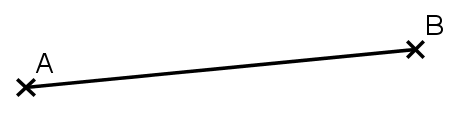
\includegraphics[width=5cm]{images/media1.png}
  \end{center}

\bigskip

  \item Construire la m�diatrice de [CD] en utilisant l'�querre. (\textit{1,5
  point})
  
\bigskip
  
  \begin{center}
  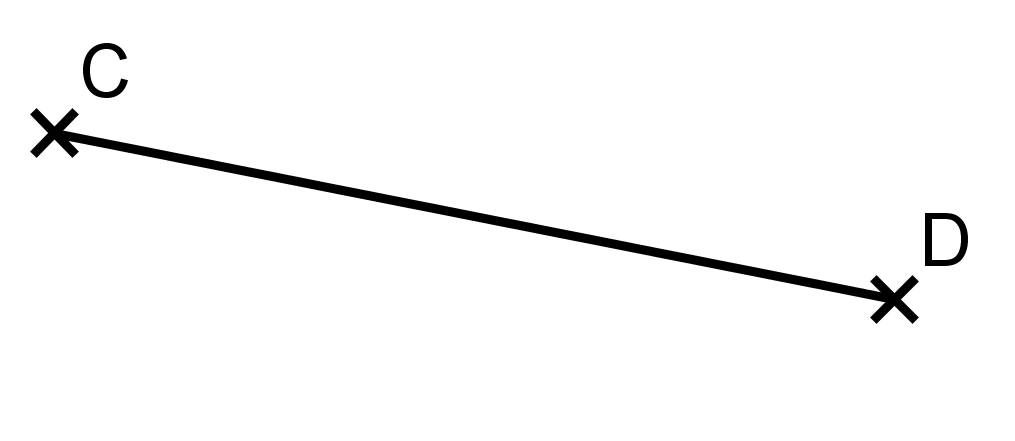
\includegraphics[width=6cm]{images/media2.png}
  \end{center}  

\bigskip
  
  \item 
  
 \begin{tabular}{cc}
 \begin{minipage}{13cm}
 DEF est un triangle rectangle en F. Tracer son cercle circonscrit (vous
  utiliserez la m�thode de votre choix).(\textit{2,5 points})

 \end{minipage}
&
 \begin{minipage}{5cm}
 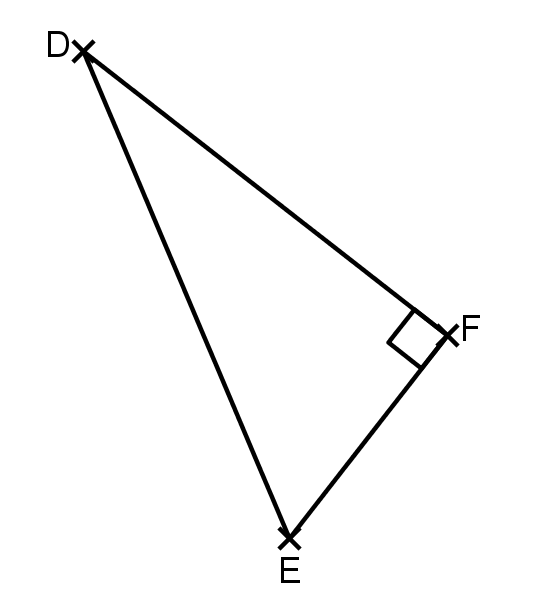
\includegraphics[width=5cm]{images/triangle2.png} 
 \end{minipage}
 \end{tabular} 
 
  
  



  \item $\mathcal{C}$ est un cercle de diam�tre [RS] et T est un point du
  cercle.
  
   \begin{tabular}{cc}
 \begin{minipage}{12cm}
 \begin{enumerate}

    \item  Que peut-on dire du triangle RST? (\textit{1 point})
    
    \rule{10cm}{0,5pt}
    
     \rule{10cm}{0,5pt}
    
    \item Citer la propri�t� du cours permettant de l'affirmer 
    
    (\textit{1,5
    point}):
    
    \rule{10cm}{0,5pt}
    
    \rule{10cm}{0,5pt} 
    
    \rule{10cm}{0,5pt}
    
    \rule{10cm}{0,5pt}
    
     \rule{10cm}{0,5pt}
     
    
  \end{enumerate}
 \end{minipage}  
&
\begin{minipage}{6cm}
 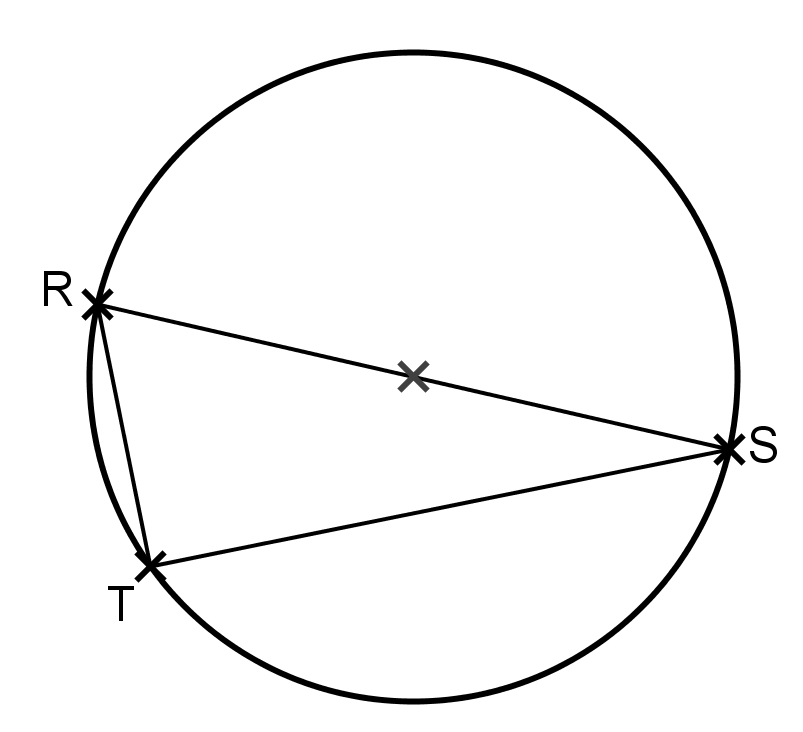
\includegraphics[width=6cm]{images/cercle2.png} 
 \end{minipage} 
\end{tabular}

  
 
  
\end{enumerate}

\end{document}
